运行 matlab/leapFrogPeriod.m 复现程序结果如下

\begin{figure}[!h]
  \caption{initial function 1}
  \centering
  \subfigure[$Q_2$]{
  \begin{minipage}[t]{0.3\linewidth}
  \centering
  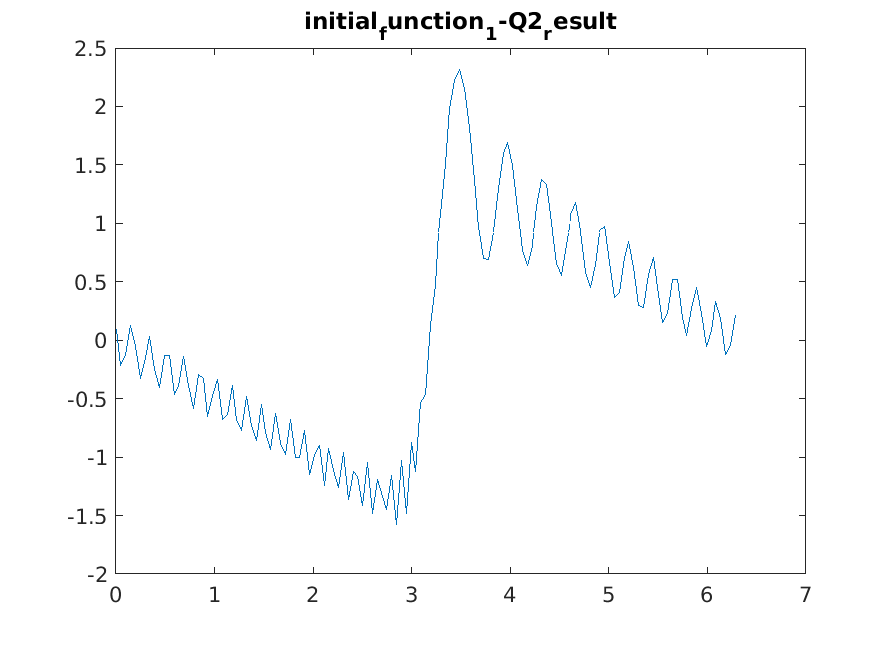
\includegraphics[height=2in, width=2in]{fig/initial_function_1-Q2_result.png}
  %\caption{fig1}
  \end{minipage}%
  }%
  \subfigure[$Q_4$]{
  \begin{minipage}[t]{0.3\linewidth}
  \centering
  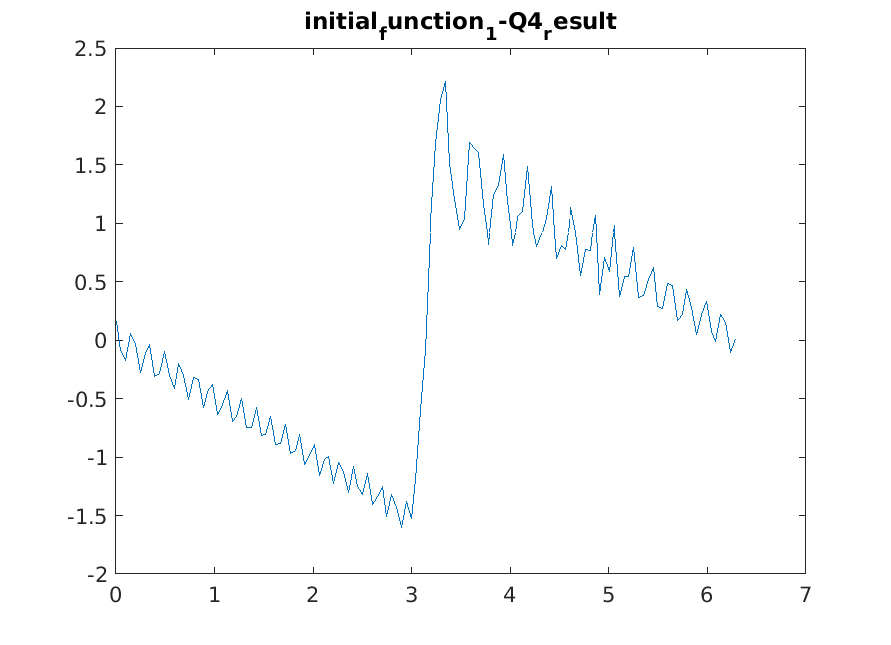
\includegraphics[height=2in, width=2in]{fig/initial_function_1-Q4_result.png}
  %\caption{fig1}
  \end{minipage}%
  }%
  \subfigure[$Q_6$]{
  \begin{minipage}[t]{0.3\linewidth}
  \centering
  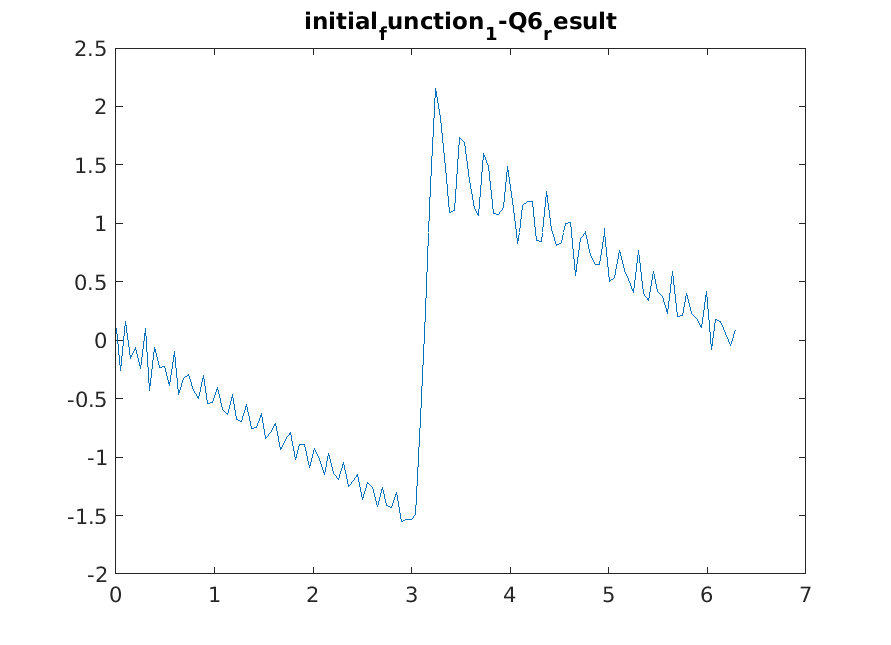
\includegraphics[height=2in, width=2in]{fig/initial_function_1-Q6_result.png}
  %\caption{fig1}
  \end{minipage}%
  }%
  
\end{figure}

\begin{figure}[!h]
  \caption{initial function 2}
  \centering
  \subfigure[$Q_2$]{
  \begin{minipage}[t]{0.3\linewidth}
  \centering
  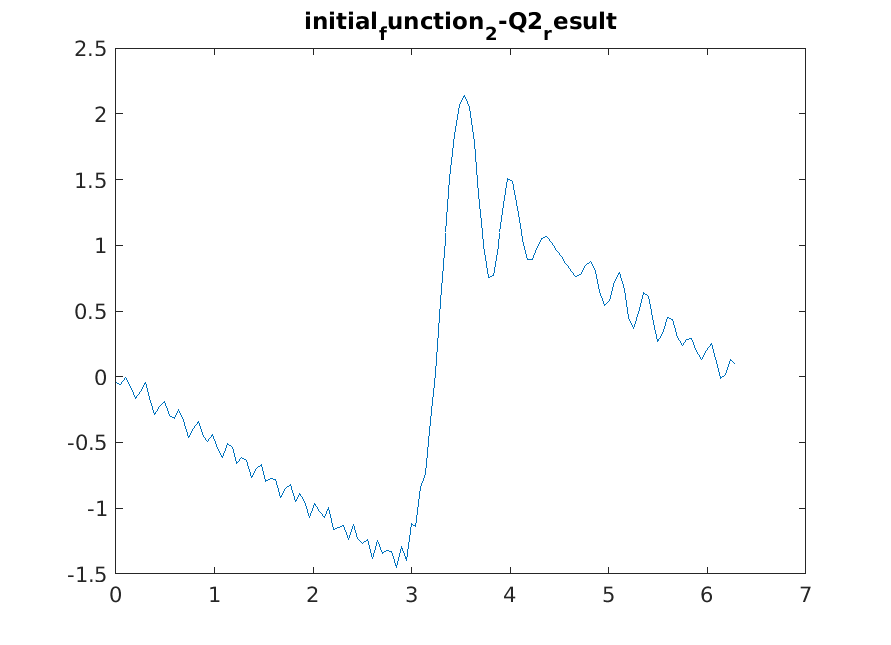
\includegraphics[height=2in, width=2in]{fig/initial_function_2-Q2_result.png}
  %\caption{fig1}
  \end{minipage}%
  }%
  \subfigure[$Q_4$]{
  \begin{minipage}[t]{0.3\linewidth}
  \centering
  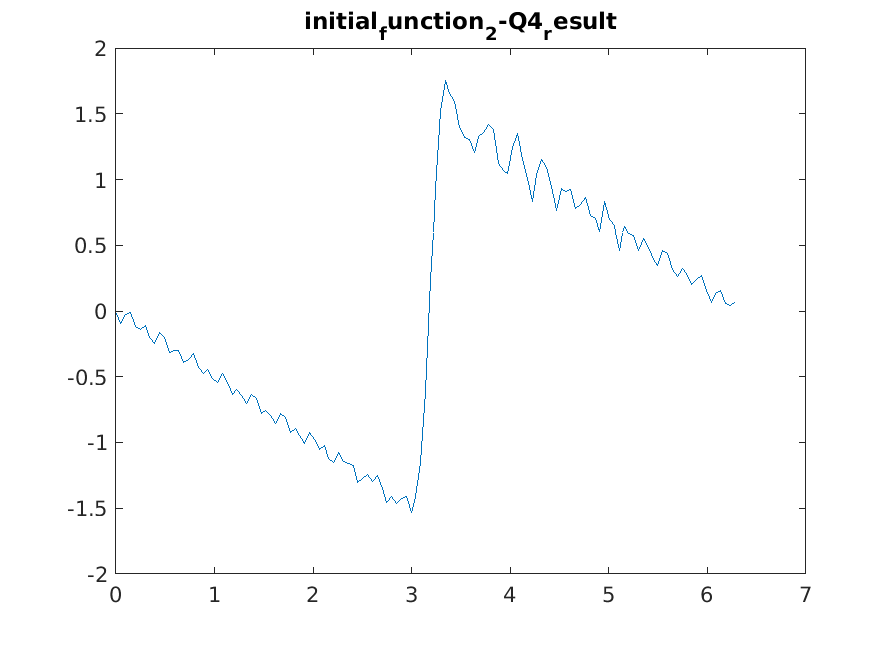
\includegraphics[height=2in, width=2in]{fig/initial_function_2-Q4_result.png}
  %\caption{fig1}
  \end{minipage}%
  }%
  \subfigure[$Q_6$]{
  \begin{minipage}[t]{0.3\linewidth}
  \centering
  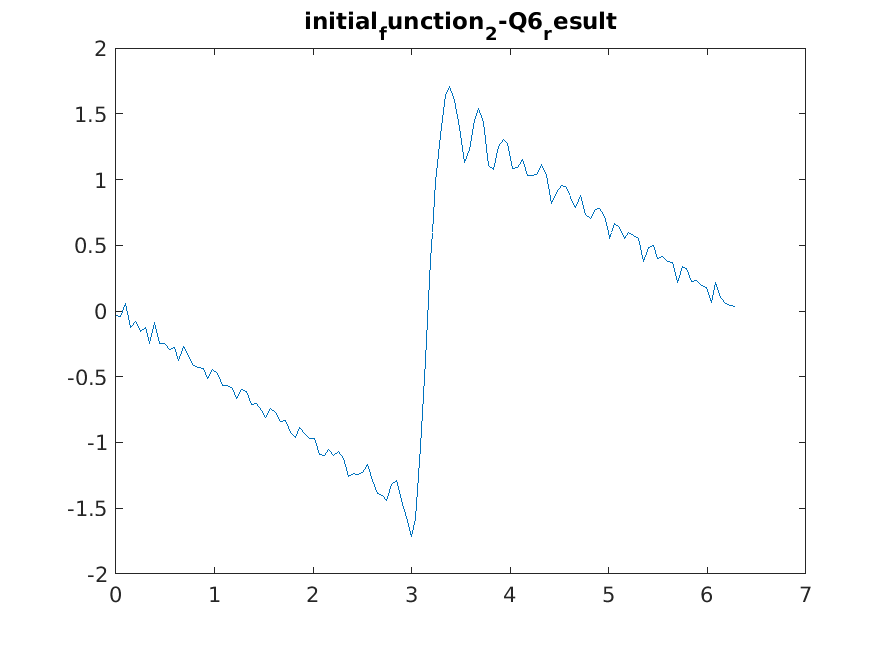
\includegraphics[height=2in, width=2in]{fig/initial_function_2-Q6_result.png}
  %\caption{fig1}
  \end{minipage}%
  }%
  
\end{figure}

\begin{figure}[!h]
  \caption{initial function 3}
  \centering
  \subfigure[$Q_2$]{
  \begin{minipage}[t]{0.3\linewidth}
  \centering
  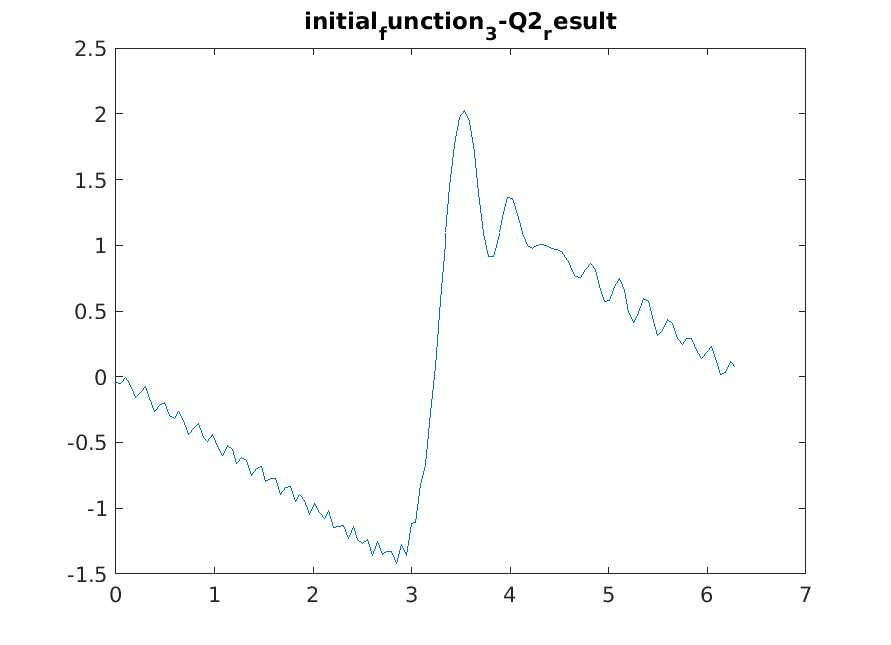
\includegraphics[height=2in, width=2in]{fig/initial_function_3-Q2_result.png}
  %\caption{fig1}
  \end{minipage}%
  }%
  \subfigure[$Q_4$]{
  \begin{minipage}[t]{0.3\linewidth}
  \centering
  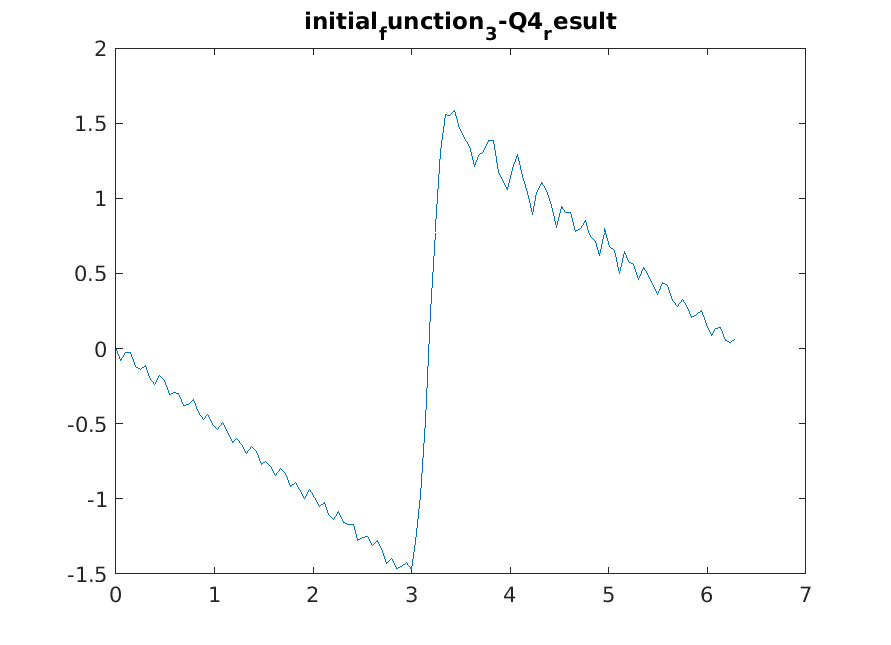
\includegraphics[height=2in, width=2in]{fig/initial_function_3-Q4_result.png}
  %\caption{fig1}
  \end{minipage}%
  }%
  \subfigure[$Q_6$]{
  \begin{minipage}[t]{0.3\linewidth}
  \centering
  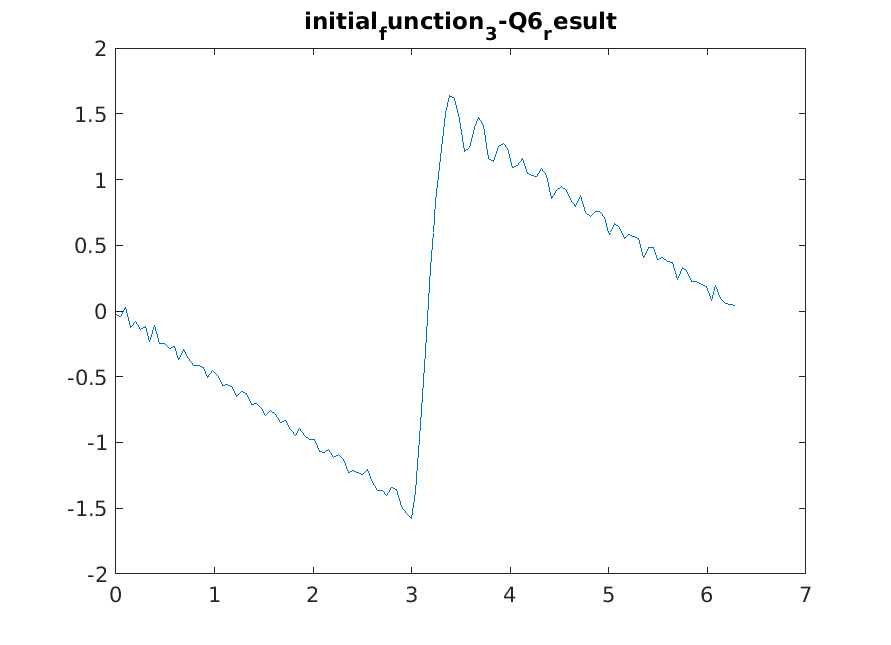
\includegraphics[height=2in, width=2in]{fig/initial_function_3-Q6_result.png}
  %\caption{fig1}
  \end{minipage}%
  }%
  
\end{figure}